% answers.tex —— 2013 年·湖南卷·理科 · 参考答案与详细解析片段
% 由 tools/generate_projects.py 依来源总账自 2013/2013_数学真题_湖南理_试题.md + 2013/2013_数学真题_湖南理_解析正文.md + 2013/2013_数学真题_湖南理_答案要点.md 生成，勿手改（改源 MD 后重跑）

\begin{answer}
\gksolhead{1}{}

\textbf{题目}：

复数 $z=\mathrm i\cdot(1+\mathrm i)$（$\mathrm i$ 为虚数单位）在复平面上对应的点位于\mbox{（　　）}

（A）第一象限；（B）第二象限；（C）第三象限；（D）第四象限。

\Needspace{4\baselineskip}
\textbf{解析}
\Needspace{5\baselineskip}
由 $\mathrm i^2=-1$，
\nopagebreak[4]
\[z=\mathrm i(1+\mathrm i)=\mathrm i+\mathrm i^2=-1+\mathrm i.\]
因此 $z$ 对应的点为 $(-1,1)$，横坐标为负、纵坐标为正，位于第二象限。选 B。

\gkanswer{答案：B。$z=-1+\mathrm i$，对应点为 $(-1,1)$，位于第二象限。}

\end{answer}
\begin{answer}
\gksolhead{2}{}

\textbf{题目}：

某学校有男、女学生各 $500$ 名。为了解男女学生在学习兴趣与业余爱好方面是否存在显著差异，拟从全体学生中抽取 $100$ 名学生进行调查，则宜采用的抽样方法是\mbox{（　　）}

（A）抽签法；（B）随机数法；（C）系统抽样法；（D）分层抽样法。

\Needspace{4\baselineskip}
\textbf{解析}
总体由男生、女生两个差异明显的部分组成，而调查目的正是比较这两部分在学习兴趣与业余爱好方面是否存在显著差异。为使样本中包含两个部分且比例合理，应按性别分层，采用分层抽样法。选 D。

\gkanswer{答案：D。男女差异明显，宜按性别分层抽取。}

\end{answer}
\begin{answer}
\gksolhead{3}{}

\textbf{题目}：

在锐角 $\triangle ABC$ 中，角 $A$，$B$ 所对的边长分别为 $a$，$b$。若 $2a\sin B=\sqrt3b$，则角 $A$ 等于\mbox{（　　）}

（A）$\dfrac{\pi}{12}$；（B）$\dfrac{\pi}{6}$；（C）$\dfrac{\pi}{4}$；（D）$\dfrac{\pi}{3}$。

\Needspace{4\baselineskip}
\textbf{解析}
\Needspace{5\baselineskip}
由正弦定理 $\dfrac{a}{\sin A}=\dfrac{b}{\sin B}$，得 $b=\dfrac{a\sin B}{\sin A}$。代入 $2a\sin B=\sqrt3b$：
\nopagebreak[4]
\[2a\sin B=\sqrt3\cdot\frac{a\sin B}{\sin A}.\]
\Needspace{5\baselineskip}
因 $a>0$，$\sin B>0$，约去后得
\nopagebreak[4]
\[\sin A=\frac{\sqrt3}{2}.\]
于是 $A=\dfrac\pi3$ 或 $A=\dfrac{2\pi}{3}$。又 $\triangle ABC$ 为锐角三角形，故只能取 $A=\dfrac\pi3$。选 D。

\gkanswer{答案：D。由正弦定理得 $\sin A=\dfrac{\sqrt3}{2}$，又三角形为锐角三角形，故 $A=\dfrac\pi3$。}

\end{answer}
\begin{answer}
\gksolhead{4}{}

\textbf{题目}：

若变量 $x$，$y$ 满足约束条件 $\begin{cases}y\leqslant 2x,\\x+y\leqslant 1,\\y\geqslant -1,\end{cases}$ 则 $x+2y$ 的最大值是\mbox{（　　）}

（A）$-\dfrac52$；（B）$0$；（C）$\dfrac53$；（D）$\dfrac52$。

\Needspace{4\baselineskip}
\textbf{解析}
\Needspace{5\baselineskip}
可行域由三条直线 $y=2x$，$x+y=1$，$y=-1$ 围成，其三个顶点为
\nopagebreak[4]
\[\left(-\frac12,-1\right),\qquad (2,-1),\qquad \left(\frac13,\frac23\right).\]
\Needspace{5\baselineskip}
分别代入 $z=x+2y$：
\nopagebreak[4]
\[z\left(-\frac12,-1\right)=-\frac52,\qquad z(2,-1)=0,\qquad z\left(\frac13,\frac23\right)=\frac13+\frac43=\frac53.\]
故最大值为 $\dfrac53$。选 C。

\gkanswer{答案：C。可行域三个顶点为 $\left(-\dfrac12,-1\right)$，$(2,-1)$，$\left(\dfrac13,\dfrac23\right)$，目标函数最大值在 $\left(\dfrac13,\dfrac23\right)$ 处取得，为 $\dfrac53$。}

\end{answer}
\begin{answer}
\gksolhead{5}{}

\textbf{题目}：

函数 $f(x)=2\ln x$ 的图象与函数 $g(x)=x^2-4x+5$ 的图象的交点个数为\mbox{（　　）}

（A）$3$；（B）$2$；（C）$1$；（D）$0$。

\Needspace{4\baselineskip}
\textbf{解析}
\Needspace{5\baselineskip}
交点个数即方程 $2\ln x=x^2-4x+5$ 在 $x>0$ 上的实根个数。令
\nopagebreak[4]
\[h(x)=x^2-4x+5-2\ln x,\]
\Needspace{5\baselineskip}
则
\nopagebreak[4]
\[h'(x)=2x-4-\frac2x=\frac{2(x^2-2x-1)}{x}.\]
\Needspace{5\baselineskip}
由 $x>0$，$h'(x)=0$ 等价于 $x^2-2x-1=0$，得唯一正根 $x_0=1+\sqrt2$。当 $0<x<x_0$ 时 $h'(x)<0$，当 $x>x_0$ 时 $h'(x)>0$，故 $h$ 在 $x_0$ 处取最小值。计算
\nopagebreak[4]
\[h(1)=1-4+5-0=2>0,\]
\nopagebreak[4]
\[h(1+\sqrt2)=(1+\sqrt2)^2-4(1+\sqrt2)+5-2\ln(1+\sqrt2)
=4-2\sqrt2-2\ln(1+\sqrt2)<0.\]
又 $x\to0^+$ 与 $x\to+\infty$ 时均有 $h(x)\to+\infty$，且 $h$ 严格凸（$h''(x)=2+\dfrac2{x^2}>0$），所以 $h$ 的图象与 $x$ 轴恰有两个交点。选 B。

\gkanswer{答案：B。令 $h(x)=x^2-4x+5-2\ln x$，其最小值 $h(1+\sqrt2)<0$，且两端趋于 $+\infty$，故有两个零点。}

\end{answer}
\begin{answer}
\gksolhead{6}{}

\textbf{题目}：

已知 $\boldsymbol a$，$\boldsymbol b$ 是单位向量，$\boldsymbol a\cdot\boldsymbol b=0$。若向量 $\boldsymbol c$ 满足 $|\boldsymbol c-\boldsymbol a-\boldsymbol b|=1$，则 $|\boldsymbol c|$ 的取值范围是\mbox{（　　）}

（A）$[\sqrt2-1,\sqrt2+1]$；（B）$[\sqrt2-1,\sqrt2+2]$；（C）$[1,\sqrt2+1]$；（D）$[1,\sqrt2+2]$。

\Needspace{4\baselineskip}
\textbf{解析}
\Needspace{5\baselineskip}
由 $\boldsymbol a\cdot\boldsymbol b=0$ 且 $|\boldsymbol a|=|\boldsymbol b|=1$，得
\nopagebreak[4]
\[|\boldsymbol a+\boldsymbol b|^2=|\boldsymbol a|^2+|\boldsymbol b|^2+2\boldsymbol a\cdot\boldsymbol b=2,\]
\Needspace{5\baselineskip}
故 $|\boldsymbol a+\boldsymbol b|=\sqrt2$。条件 $|\boldsymbol c-(\boldsymbol a+\boldsymbol b)|=1$ 表示点 $C$ 在以 $\boldsymbol a+\boldsymbol b$ 的终点为圆心、半径为 $1$ 的圆上。由三角不等式，
\nopagebreak[4]
\[\bigl||\boldsymbol c|-|\boldsymbol a+\boldsymbol b|\bigr|\leqslant|\boldsymbol c-(\boldsymbol a+\boldsymbol b)|=1,\]
\Needspace{5\baselineskip}
即
\nopagebreak[4]
\[\sqrt2-1\leqslant|\boldsymbol c|\leqslant\sqrt2+1.\]
两个端点均可取到。选 A。

\gkanswer{答案：A。$|\boldsymbol a+\boldsymbol b|=\sqrt2$，由 $|\boldsymbol c-(\boldsymbol a+\boldsymbol b)|=1$ 得 $|\boldsymbol c|\in[\sqrt2-1,\sqrt2+1]$。}

\end{answer}
\begin{answer}
\gksolhead{7}{}

\textbf{题目}：

已知棱长为 $1$ 的正方体的俯视图是一个面积为 $1$ 的正方形，则该正方体的正视图的面积不可能等于\mbox{（　　）}

（A）$1$；（B）$\sqrt2$；（C）$\dfrac{\sqrt2-1}{2}$；（D）$\dfrac{\sqrt2+1}{2}$。

\Needspace{4\baselineskip}
\textbf{解析}
\Needspace{5\baselineskip}
正方体棱长为 $1$。俯视图是面积为 $1$ 的正方形，而正方体在水平面上的正投影面积等于三个互相垂直面的投影面积之和；每项不超过 $1$，总和为 $1$ 只能是一项为 $1$、另两项为 $0$。因此正方体有一个面水平，正视图就是该水平正方形沿水平方向投影后所得矩形的面积：高恒为 $1$，宽为该正方形在正视图方向上的投影长度。设该方向与正方形一边的夹角为 $\theta$，则宽为
\nopagebreak[4]
\[\cos\theta+\sin\theta=\sqrt2\sin\left(\theta+\frac\pi4\right),\qquad 0\leqslant\theta\leqslant\frac\pi2,\]
其取值范围为 $[1,\sqrt2]$。所以正视图面积的范围是 $[1,\sqrt2]$。四个选项中，$\dfrac{\sqrt2-1}{2}<1$，不可能等于。选 C。

\gkanswer{答案：C。俯视图为面积 $1$ 的正方形时，正视图面积的范围是 $[1,\sqrt2]$，而 $\dfrac{\sqrt2-1}{2}<1$。}

\end{answer}
\begin{answer}
\gksolhead{8}{}

\textbf{题目}：

在等腰直角三角形 $ABC$ 中，$AB=AC=4$，点 $P$ 是边 $AB$ 上异于 $A$，$B$ 的一点，光线从点 $P$ 出发，经 $BC$，$CA$ 反射后又回到点 $P$（如图）。若光线 $QR$ 经过 $\triangle ABC$ 的重心，则 $AP$ 等于\mbox{（　　）}
\nopagebreak[4]
\begin{center}% 2013 湖南卷理科第 8 题：等腰直角三角形中的光线反射（TikZ 矢量重绘）。
% A(0,0), B(4,0), C(0,4)，P(4/3,0)，Q(20/9,16/9) 在 BC 上，R(0,2/3) 在 CA 上；
% 光线 P->Q->R->P，QR 经过重心 G(4/3,4/3)。
\begin{tikzpicture}[scale=1.05, font=\small, >=Stealth, line width=0.6pt]
  \coordinate (A) at (0,0);
  \coordinate (B) at (4,0);
  \coordinate (C) at (0,4);
  \coordinate (P) at (1.3333,0);
  \coordinate (Q) at (2.2222,1.7778);
  \coordinate (R) at (0,0.6667);
  \coordinate (G) at (1.3333,1.3333);

  \draw (A) -- (B) -- (C) -- cycle;

  \draw[->] (P) -- (Q);
  \draw[->] (Q) -- (R);
  \draw[->] (R) -- (P);

  \fill (G) circle (1.4pt);
  \node[above right] at (G) {$G$};

  \node[below left] at (A) {$A$};
  \node[below right] at (B) {$B$};
  \node[above left] at (C) {$C$};
  \node[below] at (P) {$P$};
  \node[right] at (Q) {$Q$};
  \node[left] at (R) {$R$};
\end{tikzpicture}
\end{center}
\nopagebreak[4]
（A）$2$；（B）$1$；（C）$\dfrac83$；（D）$\dfrac43$。

\Needspace{4\baselineskip}
\textbf{解析}
\Needspace{5\baselineskip}
以 $A$ 为原点，$AB$ 为 $x$ 轴，$AC$ 为 $y$ 轴建立坐标系，则
\nopagebreak[4]
\[A(0,0),\quad B(4,0),\quad C(0,4),\quad G\left(\frac43,\frac43\right).\]
设 $P(p,0)$（$0<p<4$），$R(0,r)$，$Q(q,4-q)$。

光线在 $CA$（即 $y$ 轴）上的 $R$ 点反射，故把 $P$ 关于 $y$ 轴反射到 $P'(-p,0)$ 后，$Q$，$R$，$P'$ 三点共线。光线在 $BC$（即 $x+y=4$）上的 $Q$ 点反射，故把 $P$ 关于直线 $x+y=4$ 反射到 $P''(4,4-p)$ 后，$P''$，$Q$，$R$ 三点共线。于是 $P'$，$Q$，$R$，$P''$ 共线，即反射折线 $PQR$ 展开后成为直线 $P'P''$。题设 $QR$ 经过重心 $G$，所以 $G$ 在直线 $P'P''$ 上。

\Needspace{5\baselineskip}
直线 $P'P''$ 经过 $(-p,0)$ 与 $(4,4-p)$。由 $G\left(\dfrac43,\dfrac43\right)$ 在其上，按纵坐标比例有
\nopagebreak[4]
\[-p+\frac{\frac43}{4-p}(4+p)=\frac43.\]
\Needspace{5\baselineskip}
两边乘以 $3(4-p)$：
\nopagebreak[4]
\[-3p(4-p)+4(4+p)=4(4-p).\]
\Needspace{5\baselineskip}
展开整理：
\nopagebreak[4]
\[-12p+3p^2+16+4p=16-4p
\Longrightarrow 3p^2-4p=0
\Longrightarrow p(3p-4)=0.\]
因 $0<p<4$，故 $p=\dfrac43$。即 $AP=\dfrac43$。选 D。

\gkanswer{答案：D。两次反射展开后，$P$ 的两个像点与重心共线，解得 $AP=\dfrac43$。}

\end{answer}
\begin{answer}
\gksolhead{9}{}

\textbf{题目}：

在平面直角坐标系 $xOy$ 中，若直线 $l:\begin{cases}x=t,\\y=t-a,\end{cases}$（$t$ 为参数）过椭圆 $C:\begin{cases}x=3\cos\varphi,\\y=2\sin\varphi,\end{cases}$（$\varphi$ 为参数）的右顶点，则常数 $a$ 的值为\gkblank{}。

\Needspace{4\baselineskip}
\textbf{解析}
\Needspace{5\baselineskip}
椭圆 $C$ 的参数方程为 $x=3\cos\varphi$，$y=2\sin\varphi$，其右顶点为 $(3,0)$。直线 $l$ 的参数方程为 $x=t$，$y=t-a$，过点 $(3,0)$ 时必须
\nopagebreak[4]
\[t=3,\qquad 0=3-a,\]
故 $a=3$。

\gkanswer{答案：$3$。椭圆右顶点为 $(3,0)$，代入 $x=t$，$y=t-a$ 得 $t=3$，$3-a=0$。}

\end{answer}
\begin{answer}
\gksolhead{10}{}

\textbf{题目}：

已知 $a$，$b$，$c\in\mathbf R$，$a+2b+3c=6$，则 $a^2+4b^2+9c^2$ 的最小值为\gkblank{}。

\Needspace{4\baselineskip}
\textbf{解析}
\Needspace{5\baselineskip}
由柯西不等式，
\nopagebreak[4]
\[(1^2+1^2+1^2)\left[a^2+(2b)^2+(3c)^2\right]\geqslant(a+2b+3c)^2=36,\]
\Needspace{5\baselineskip}
即
\nopagebreak[4]
\[a^2+4b^2+9c^2\geqslant\frac{36}{3}=12.\]
当 $a=2b=3c$ 且 $a+2b+3c=6$ 时取等号，例如 $a=2$，$b=1$，$c=\dfrac23$。故最小值为 $12$。

\gkanswer{答案：$12$。由柯西不等式 $(1+1+1)(a^2+4b^2+9c^2)\geqslant(a+2b+3c)^2=36$。}

\end{answer}
\begin{answer}
\gksolhead{11}{}

\textbf{题目}：

如图，在半径为 $\sqrt7$ 的 $\odot O$ 中，弦 $AB$，$CD$ 相交于点 $P$，$PA=PB=2$，$PD=1$，则圆心 $O$ 到弦 $CD$ 的距离为\gkblank{}。
\nopagebreak[4]
\begin{center}% 2013 湖南卷理科第 11 题：圆 O 中弦 AB 与 CD 交于 P（TikZ 矢量重绘）。
% 半径 sqrt(7)，P(0,sqrt3)，A(-2,sqrt3)，B(2,sqrt3)，D(1/2,3sqrt3/2)，C(-2,-sqrt3)。
% 此时 PA=PB=2，PD=1，PC=4，CD=5。
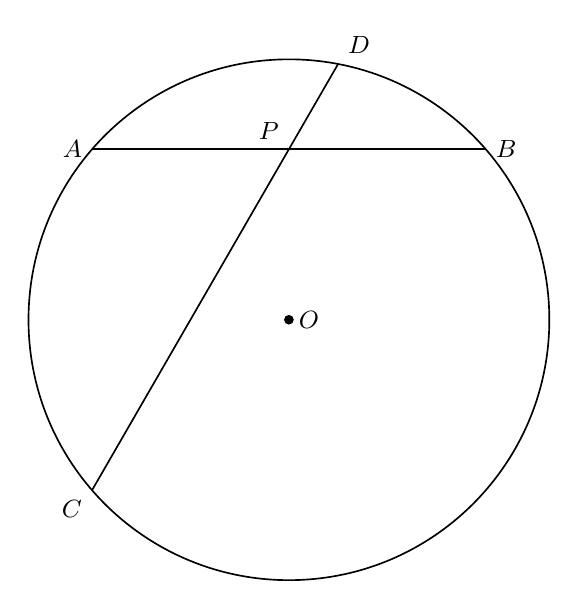
\begin{tikzpicture}[scale=1.25, font=\small, line width=0.6pt]
  \coordinate (O) at (0,0);
  \coordinate (P) at (0,1.7321);
  \coordinate (A) at (-2,1.7321);
  \coordinate (B) at (2,1.7321);
  \coordinate (D) at (0.5,2.5981);
  \coordinate (C) at (-2,-1.7321);

  \draw (O) circle ({sqrt(7)});
  \draw (A) -- (B);
  \draw (C) -- (D);

  \fill (O) circle (1.4pt);
  \node[right] at (O) {$O$};
  \node[above left] at (P) {$P$};
  \node[left] at (A) {$A$};
  \node[right] at (B) {$B$};
  \node[above right] at (D) {$D$};
  \node[below left] at (C) {$C$};
\end{tikzpicture}
\end{center}
\nopagebreak[4]
\Needspace{4\baselineskip}
\textbf{解析}
\Needspace{5\baselineskip}
由相交弦定理，
\nopagebreak[4]
\[PA\cdot PB=PC\cdot PD.\]
\Needspace{5\baselineskip}
代入 $PA=PB=2$，$PD=1$，得
\nopagebreak[4]
\[2\cdot2=PC\cdot1\Longrightarrow PC=4.\]
\Needspace{5\baselineskip}
所以弦 $CD$ 的长为
\nopagebreak[4]
\[CD=PC+PD=4+1=5.\]
\Needspace{5\baselineskip}
设圆心 $O$ 到弦 $CD$ 的距离为 $d$。由垂径定理与勾股定理，
\nopagebreak[4]
\[d^2+\left(\frac{CD}{2}\right)^2=R^2=7,\]
\Needspace{5\baselineskip}
故
\nopagebreak[4]
\[d=\sqrt{7-\left(\frac52\right)^2}=\sqrt{7-\frac{25}{4}}=\frac{\sqrt3}{2}.\]

\gkanswer{答案：$\dfrac{\sqrt3}{2}$。由相交弦定理 $PC\cdot PD=PA\cdot PB$ 得 $PC=4$，故 $CD=5$，圆心到 $CD$ 的距离为 $\sqrt{7-\left(\dfrac52\right)^2}$。}

\end{answer}
\begin{answer}
\gksolhead{12}{}

\textbf{题目}：

若 $\displaystyle\int_0^T x^2\,\mathrm dx=9$，则常数 $T$ 的值为\gkblank{}。

\Needspace{4\baselineskip}
\textbf{解析}
\nopagebreak[4]
\[\int_0^T x^2\,\mathrm dx=\left[\frac{x^3}{3}\right]_0^T=\frac{T^3}{3}.\]
由 $\dfrac{T^3}{3}=9$ 得 $T^3=27$，故 $T=3$。

\gkanswer{答案：$3$。$\displaystyle\int_0^T x^2\,\mathrm dx=\dfrac{T^3}{3}=9$，故 $T^3=27$。}

\end{answer}
\begin{answer}
\gksolhead{13}{}

\textbf{题目}：

执行如图所示的程序框图，如果输入 $a=1$，$b=2$，则输出的 $a$ 的值为\gkblank{}。
\nopagebreak[4]
\begin{center}% 2013 湖南卷理科第 13 题：程序框图（TikZ 矢量重绘）。
% 输入 a=1, b=2；判断 a>8？是则输出 a，否则 a=a+b 后返回判断。
\begin{tikzpicture}[font=\footnotesize, >=Stealth, line width=0.5pt,
  box/.style={draw, minimum height=1.9em, inner xsep=8pt},
  term/.style={draw, rounded corners=6pt, minimum height=1.9em, inner xsep=10pt},
  io/.style={draw, trapezium, trapezium left angle=70, trapezium right angle=110,
             minimum height=1.9em, inner xsep=8pt},
  dec/.style={draw, diamond, aspect=2.4, inner sep=1.5pt}]

  \node[term] (start) at (0,0) {开始};
  \node[io]   (in)    at (0,-1.5) {输入 $a$，$b$};
  \node[dec]  (test)  at (0,-3.6) {$a>8$?};
  \node[box]  (add)   at (0,-5.9) {$a=a+b$};
  \node[io]   (out)   at (4.4,-3.6) {输出 $a$};
  \node[term] (end)   at (4.4,-5.3) {结束};

  \draw[->] (start) -- (in);
  \draw[->] (in) -- (test);
  \draw[->] (test) -- node[left] {否} (add);
  \draw[->] (test) -- node[above] {是} (out);
  \draw[->] (out) -- (end);
  \draw[->] (add.west) -- (-2.2,-5.9) -- (-2.2,-2.6) -- (test.west);
\end{tikzpicture}
\end{center}
\nopagebreak[4]
\Needspace{4\baselineskip}
\textbf{解析}
\Needspace{5\baselineskip}
初始 $a=1$，$b=2$。每次判断 $a>8$：若否，则执行 $a=a+b$ 后返回判断。依次得到
\nopagebreak[4]
\[a=1\ \xrightarrow{\text{\text{否}}}\ 3\ \xrightarrow{\text{\text{否}}}\ 5\ \xrightarrow{\text{\text{否}}}\ 7\ \xrightarrow{\text{\text{否}}}\ 9.\]
当 $a=9$ 时 $9>8$ 成立，输出 $a=9$。

\gkanswer{答案：$9$。$a$ 依次取 $1,3,5,7,9$，当 $a=9$ 时满足 $a>8$，输出 $9$。}

\end{answer}
\begin{answer}
\gksolhead{14}{}

\textbf{题目}：

设 $F_1$，$F_2$ 是双曲线 $C:\dfrac{x^2}{a^2}-\dfrac{y^2}{b^2}=1$（$a>0$，$b>0$）的两个焦点，$P$ 是 $C$ 上一点，若 $|PF_1|+|PF_2|=6a$，且 $\triangle PF_1F_2$ 的最小内角为 $30^\circ$，则 $C$ 的离心率为\gkblank{}。

\Needspace{4\baselineskip}
\textbf{解析}
\Needspace{5\baselineskip}
设 $|PF_1|=m$，$|PF_2|=n$。由双曲线定义，
\nopagebreak[4]
\[|m-n|=2a,\]
\Needspace{5\baselineskip}
又题设 $m+n=6a$，故 $\{m,n\}=\{4a,2a\}$。于是 $\triangle PF_1F_2$ 的三边为
\nopagebreak[4]
\[2a,\quad 4a,\quad 2c.\]
\Needspace{5\baselineskip}
其中最短边为 $2a$，故最小内角 $30^\circ$ 是 $2a$ 所对的角。由余弦定理，
\nopagebreak[4]
\[\cos30^\circ=\frac{(4a)^2+(2c)^2-(2a)^2}{2\cdot4a\cdot2c}
=\frac{12a^2+4c^2}{16ac}
=\frac{3a^2+c^2}{4ac}.\]
\Needspace{5\baselineskip}
代入 $\cos30^\circ=\dfrac{\sqrt3}{2}$：
\nopagebreak[4]
\[\frac{3a^2+c^2}{4ac}=\frac{\sqrt3}{2}
\Longrightarrow 3a^2+c^2=2\sqrt3ac
\Longrightarrow (c-\sqrt3a)^2=0.\]
\Needspace{5\baselineskip}
故 $c=\sqrt3a$，离心率
\nopagebreak[4]
\[e=\frac ca=\sqrt3.\]

\gkanswer{答案：$\sqrt3$。由双曲线定义得 $|PF_1|$，$|PF_2|$ 为 $4a$，$2a$，最小角所对边为 $2a$，由余弦定理得 $(c-\sqrt3a)^2=0$。}

\end{answer}
\begin{answer}
\gksolhead{15}{}

\textbf{题目}：

设 $S_n$ 为数列 $\{a_n\}$ 的前 $n$ 项和，$S_n=(-1)^na_n-\dfrac1{2^n}$，$n\in\mathbf N^*$，则

（1） $a_3=$\gkblank{}；

（2） $S_1+S_2+\cdots+S_{100}=$\gkblank{}。

\Needspace{4\baselineskip}
\textbf{解析}
\Needspace{5\baselineskip}
\textbf{（1）} 当 $n\geqslant2$ 时，由 $a_n=S_n-S_{n-1}$ 及题设
\nopagebreak[4]
\[S_n=(-1)^na_n-\frac1{2^n},\qquad
S_{n-1}=(-1)^{n-1}a_{n-1}-\frac1{2^{n-1}},\]
\Needspace{5\baselineskip}
得
\nopagebreak[4]
\[a_n=(-1)^na_n-(-1)^{n-1}a_{n-1}-\frac1{2^n}+\frac1{2^{n-1}}
=(-1)^na_n+(-1)^na_{n-1}+\frac1{2^n}.\]
\Needspace{5\baselineskip}
取 $n=4$（偶数），则 $(-1)^4=1$，上式化为
\nopagebreak[4]
\[a_4=a_4+a_3+\frac1{16}\Longrightarrow a_3=-\frac1{16}.\]

\textbf{（2）} 由（1）中的递推式：
\begin{itemize}
\item 当 $n$ 为偶数时，$a_{n-1}=-\dfrac1{2^n}$；
\item 当 $n$ 为奇数时，$2a_n+a_{n-1}=\dfrac1{2^n}$。
\end{itemize}

\Needspace{5\baselineskip}
由偶数情形，取 $n=2k$ 得
\nopagebreak[4]
\[a_{2k-1}=-\frac1{2^{2k}}=-\frac1{4^k}.\]
\Needspace{5\baselineskip}
再由奇数情形求偶数项：
\nopagebreak[4]
\[2a_{2k+1}+a_{2k}=\frac1{2^{2k+1}},\qquad
a_{2k+1}=-\frac1{4^{k+1}},\]
\Needspace{5\baselineskip}
故
\nopagebreak[4]
\[a_{2k}=\frac1{2^{2k+1}}+\frac2{4^{k+1}}
=\frac1{2\cdot4^k}+\frac1{2\cdot4^k}=\frac1{4^k}.\]
\Needspace{5\baselineskip}
于是
\nopagebreak[4]
\[S_{2k-1}=(-1)^{2k-1}a_{2k-1}-\frac1{2^{2k-1}}
=\frac1{4^k}-\frac2{4^k}=-\frac1{4^k},\]
\nopagebreak[4]
\[S_{2k}=a_{2k}-\frac1{2^{2k}}=\frac1{4^k}-\frac1{4^k}=0.\]
\Needspace{5\baselineskip}
所以
\nopagebreak[4]
\[S_1+S_2+\cdots+S_{100}
=\sum_{k=1}^{50}S_{2k-1}+\sum_{k=1}^{50}S_{2k}
=-\sum_{k=1}^{50}\frac1{4^k}
=-\frac{\frac14\left(1-\frac1{4^{50}}\right)}{1-\frac14}
=\frac{2^{-100}-1}{3}.\]

\gkanswer{答案（1）：$-\dfrac1{16}$。由 $S_n-S_{n-1}=a_n$ 得 $n=4$ 时 $a_3=-\dfrac1{2^4}$。}

\gkanswer{答案（2）：$\dfrac{2^{-100}-1}{3}$。$S_{2k-1}=-\dfrac1{4^k}$，$S_{2k}=0$，故总和为 $-\displaystyle\sum_{k=1}^{50}\dfrac1{4^k}$。}

\end{answer}
\begin{answer}
\gksolhead{16}{}

\textbf{题目}：

设函数 $f(x)=a^x+b^x-c^x$，其中 $c>a>0$，$c>b>0$。

（1） 记集合 $M$ 由满足 $a=b$ 且 $a,b,c$ 不能构成一个三角形的三条边长的有序三元组 $(a,b,c)$ 组成，则 $(a,b,c)\in M$ 所对应的 $f(x)$ 的零点的取值集合为\gkblank{}；

（2） 若 $a$，$b$，$c$ 是 $\triangle ABC$ 的三条边长，则下列结论正确的是\gkblank{}。（写出所有正确结论的序号）

① $\forall x\in(-\infty,1)$，$f(x)>0$；

② $\exists x\in\mathbf R$，使 $a^x$，$b^x$，$c^x$ 不能构成一个三角形的三条边长；

③ 若 $\triangle ABC$ 为钝角三角形，则 $\exists x\in(1,2)$，使 $f(x)=0$。

\Needspace{4\baselineskip}
\textbf{解析}
\Needspace{5\baselineskip}
\textbf{（1）} 当 $a=b$ 时，$f(x)=2a^x-c^x$。$f(x)=0$ 等价于
\nopagebreak[4]
\[\left(\frac ca\right)^x=2.\]
\Needspace{5\baselineskip}
又 $a,b,c$ 不能构成三角形且 $c$ 最大，故 $a+b\leqslant c$，即 $c\geqslant2a$，从而 $\dfrac ca\geqslant2$。于是
\nopagebreak[4]
\[x=\log_{c/a}2,\qquad 0<x\leqslant1,\]
且当 $c/a$ 取遍 $[2,+\infty)$ 时 $x$ 取遍 $(0,1]$。故零点取值集合为 $(0,1]$。

\textbf{（2）} 设 $a,b,c$ 是三角形三边。因 $c>a$，$c>b$，故 $c$ 为最大边，且 $a+b>c$。

\Needspace{5\baselineskip}
① 当 $x<1$ 时，由 $0<\dfrac ac<1$，$0<\dfrac bc<1$ 及指数函数的单调性，
\nopagebreak[4]
\[\left(\frac ac\right)^x>\frac ac,\qquad
\left(\frac bc\right)^x>\frac bc.\]
\Needspace{5\baselineskip}
相加得
\nopagebreak[4]
\[\left(\frac ac\right)^x+\left(\frac bc\right)^x>\frac{a+b}{c}>1.\]
\Needspace{5\baselineskip}
因此
\nopagebreak[4]
\[f(x)=c^x\left[\left(\frac ac\right)^x+\left(\frac bc\right)^x-1\right]>0.\]
①正确。

\Needspace{5\baselineskip}
② 因 $0<\dfrac ac<1$，$0<\dfrac bc<1$，当 $x\to+\infty$ 时，
\nopagebreak[4]
\[\left(\frac ac\right)^x+\left(\frac bc\right)^x\to0.\]
故存在充分大的 $x$，使 $a^x+b^x<c^x$，此时 $a^x$，$b^x$，$c^x$ 不能构成三角形。②正确。

\Needspace{5\baselineskip}
③ 若 $\triangle ABC$ 为钝角三角形，因 $c$ 为最大边，钝角必为 $c$ 所对的角，故
\nopagebreak[4]
\[c^2>a^2+b^2.\]
\Needspace{5\baselineskip}
于是
\nopagebreak[4]
\[f(1)=a+b-c>0,\qquad f(2)=a^2+b^2-c^2<0.\]
$f$ 在 $[1,2]$ 上连续，由零点存在定理，存在 $x\in(1,2)$ 使 $f(x)=0$。③正确。

综上，正确的是①②③。

\gkanswer{答案（1）：$(0,1]$。$a=b$ 且不能构成三角形时 $c\geqslant2a$，由 $2a^x=c^x$ 得 $x=\log_{c/a}2\in(0,1]$。}

\gkanswer{答案（2）：①②③。①由 $(a/c)^x+(b/c)^x>(a+b)/c>1$；②取 $x$ 充分大；③由 $f(1)>0$，$f(2)=a^2+b^2-c^2<0$ 及零点存在定理。}

\end{answer}
\begin{answer}
\gksolhead{17}{}

\textbf{题目}：

已知函数 $f(x)=\sin\left(x-\dfrac{\pi}{6}\right)+\cos\left(x-\dfrac{\pi}{3}\right)$，$g(x)=2\sin^2\dfrac x2$。

（1） 若 $\alpha$ 是第一象限角，且 $f(\alpha)=\dfrac{3\sqrt3}{5}$，求 $g(\alpha)$ 的值；

（2） 求使 $f(x)\geqslant g(x)$ 成立的 $x$ 的取值集合。

\Needspace{4\baselineskip}
\textbf{解析}
\Needspace{5\baselineskip}
\textbf{（1）} 先化简 $f(x)$：
\nopagebreak[4]
\[\begin{aligned}
f(x)&=\sin\left(x-\frac\pi6\right)+\cos\left(x-\frac\pi3\right)\\
&=\left(\frac{\sqrt3}{2}\sin x-\frac12\cos x\right)
+\left(\frac12\cos x+\frac{\sqrt3}{2}\sin x\right)\\
&=\sqrt3\sin x.
\end{aligned}\]
\Needspace{5\baselineskip}
由 $f(\alpha)=\dfrac{3\sqrt3}{5}$ 得
\nopagebreak[4]
\[\sqrt3\sin\alpha=\frac{3\sqrt3}{5}\Longrightarrow\sin\alpha=\frac35.\]
\Needspace{5\baselineskip}
$\alpha$ 为第一象限角，故
\nopagebreak[4]
\[\cos\alpha=\sqrt{1-\sin^2\alpha}=\frac45.\]
\Needspace{5\baselineskip}
于是
\nopagebreak[4]
\[g(\alpha)=2\sin^2\frac\alpha2=1-\cos\alpha=\frac15.\]

\Needspace{5\baselineskip}
\textbf{（2）} 不等式 $f(x)\geqslant g(x)$ 即
\nopagebreak[4]
\[\sqrt3\sin x\geqslant2\sin^2\frac x2=1-\cos x.\]
\Needspace{5\baselineskip}
移项得
\nopagebreak[4]
\[\sqrt3\sin x+\cos x\geqslant1.\]
\Needspace{5\baselineskip}
左边合并：
\nopagebreak[4]
\[2\sin\left(x+\frac\pi6\right)\geqslant1
\Longrightarrow\sin\left(x+\frac\pi6\right)\geqslant\frac12.\]
\Needspace{5\baselineskip}
所以
\nopagebreak[4]
\[\frac\pi6+2k\pi\leqslant x+\frac\pi6\leqslant\frac{5\pi}{6}+2k\pi,\qquad k\in\mathbf Z,\]
\Needspace{5\baselineskip}
即
\nopagebreak[4]
\[2k\pi\leqslant x\leqslant2k\pi+\frac{2\pi}{3},\qquad k\in\mathbf Z.\]
\Needspace{5\baselineskip}
所求集合为
\nopagebreak[4]
\[\left\{x\left|2k\pi\leqslant x\leqslant2k\pi+\frac{2\pi}{3},\ k\in\mathbf Z\right.\right\}.\]

\gkanswer{答案（1）：$\dfrac15$。$f(x)=\sqrt3\sin x$，由 $f(\alpha)=\dfrac{3\sqrt3}{5}$ 得 $\sin\alpha=\dfrac35$，$\cos\alpha=\dfrac45$，故 $g(\alpha)=1-\cos\alpha=\dfrac15$。}

\gkanswer{答案（2）：$\left\{x\left|2k\pi\leqslant x\leqslant2k\pi+\dfrac{2\pi}{3},\ k\in\mathbf Z\right.\right\}$。不等式化为 $\sin\left(x+\dfrac\pi6\right)\geqslant\dfrac12$。}

\end{answer}
\begin{answer}
\gksolhead{18}{}

\textbf{题目}：

某人在如图所示的直角边长为 $4$ 米的三角形地块的每个格点（指纵、横直线的交叉点以及三角形的顶点）处都种了一株相同品种的作物。根据历年的种植经验，一株该种作物的年收获量 $Y$（单位：$\mathrm{kg}$）与它的“相近”作物株数 $X$ 之间的关系如下表所示：

\begin{center}
\begin{tabular}{lllll}
\toprule
$X$ & 1 & 2 & 3 & 4 \\
\midrule
$Y$ & 51 & 48 & 45 & 42 \\
\bottomrule
\end{tabular}
\end{center}

这里，两株作物“相近”是指它们之间的直线距离不超过 $1$ 米。

（1） 从三角形地块的内部和边界上分别随机选取一株作物，求它们恰好“相近”的概率；

（2） 从所种作物中随机选取一株，求它的年收获量的分布列与数学期望。
\nopagebreak[4]
\begin{center}% 2013 湖南卷理科第 18 题：直角边长 4 米的三角形地块及格点作物（TikZ 矢量重绘）。
% 格点为满足 x,y>=0, x+y<=4 的整点，共 15 个。
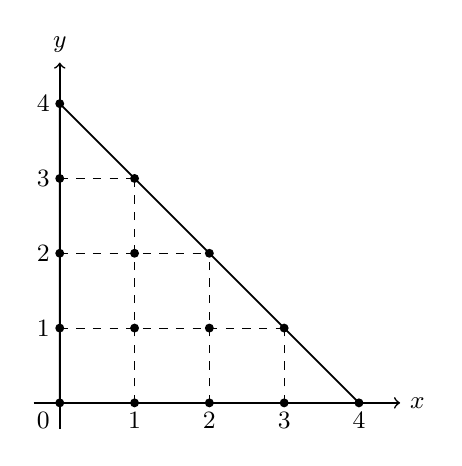
\begin{tikzpicture}[scale=0.95, font=\small, line width=0.6pt]
  \draw[->] (-0.35,0) -- (4.55,0) node[right] {$x$};
  \draw[->] (0,-0.35) -- (0,4.55) node[above] {$y$};
  \node[below left] at (0,0) {$0$};

  \begin{scope}
    \clip (0,0) -- (4,0) -- (0,4) -- cycle;
    \foreach \i in {1,2,3} {
      \draw[dashed, line width=0.35pt] (\i,0) -- (\i,4);
      \draw[dashed, line width=0.35pt] (0,\i) -- (4,\i);
    }
  \end{scope}

  \draw (0,0) -- (4,0) -- (0,4) -- cycle;

  \foreach \x in {1,2,3,4} {
    \node[below] at (\x,0) {$\x$};
    \node[left] at (0,\x) {$\x$};
  }
  \foreach \x in {0,...,4} {
    \foreach \y in {0,...,4} {
      \ifnum\numexpr\x+\y\relax<5
        \fill (\x,\y) circle (1.7pt);
      \fi
    }
  }
\end{tikzpicture}
\end{center}
\nopagebreak[4]
\Needspace{4\baselineskip}
\textbf{解析}
\Needspace{5\baselineskip}
三角形地块内的格点为满足 $x,y\in\mathbf Z$，$x\geqslant0$，$y\geqslant0$，$x+y\leqslant4$ 的点，共
\nopagebreak[4]
\[\frac{5\times6}{2}=15\]
\Needspace{5\baselineskip}
个。其中严格位于内部的格点（$x\geqslant1$，$y\geqslant1$，$x+y<4$）为
\nopagebreak[4]
\[(1,1),\quad(1,2),\quad(2,1),\]
共 $3$ 个；边界格点共 $15-3=12$ 个。

\textbf{（1）} 从内部、边界各随机取一株，共有 $3\times12=36$ 个等可能的有序点对。逐一数出与内部点直线距离不超过 $1$ 的边界点：

\begin{itemize}
\item 与 $(1,1)$ 相近的边界点：$(1,0)$，$(0,1)$，共 $2$ 个；
\item 与 $(1,2)$ 相近的边界点：$(0,2)$，$(1,3)$，$(2,2)$，共 $3$ 个；
\item 与 $(2,1)$ 相近的边界点：$(2,0)$，$(3,1)$，$(2,2)$，共 $3$ 个。
\end{itemize}

\Needspace{5\baselineskip}
有利点对共 $2+3+3=8$ 个，故所求概率为
\nopagebreak[4]
\[P=\frac{8}{36}=\frac29.\]

\textbf{（2）} 对全部 $15$ 个格点，统计每个格点周围距离不超过 $1$ 的格点数 $X$：

\begin{itemize}
\item $X=1$：$(0,4)$，$(4,0)$，共 $2$ 个；
\item $X=2$：$(0,0)$，$(1,3)$，$(2,2)$，$(3,1)$，共 $4$ 个；
\item $X=3$：$(0,1)$，$(0,2)$，$(0,3)$，$(1,0)$，$(2,0)$，$(3,0)$，共 $6$ 个；
\item $X=4$：$(1,1)$，$(1,2)$，$(2,1)$，共 $3$ 个。
\end{itemize}

\Needspace{5\baselineskip}
合计 $2+4+6+3=15$。由题表，$X=1,2,3,4$ 分别对应 $Y=51,48,45,42$，故 $Y$ 的分布列为
\nopagebreak[4]
\[\begin{aligned}
P(Y=51)&=\frac2{15},\qquad P(Y=48)=\frac4{15},\\
P(Y=45)&=\frac6{15}=\frac25,\qquad P(Y=42)=\frac3{15}=\frac15.
\end{aligned}\]
\Needspace{5\baselineskip}
数学期望为
\nopagebreak[4]
\[E(Y)=51\cdot\frac2{15}+48\cdot\frac4{15}+45\cdot\frac6{15}+42\cdot\frac3{15}
=\frac{102+192+270+126}{15}
=\frac{690}{15}=46.\]

\gkanswer{答案（1）：$\dfrac29$。内部格点 $3$ 个，边界格点 $12$ 个，恰“相近”的有序点对为 $8$ 对，概率为 $\dfrac8{3\times12}$。}

\gkanswer{答案（2）：$P(Y=51)=\dfrac2{15}$，$P(Y=48)=\dfrac4{15}$，$P(Y=45)=\dfrac25$，$P(Y=42)=\dfrac15$；$E(Y)=46$。}

\end{answer}
\begin{answer}
\gksolhead{19}{}

\textbf{题目}：

如图，在直棱柱 $ABCD-A_1B_1C_1D_1$ 中，$AD\parallel BC$，$\angle BAD=90^\circ$，$AC\perp BD$，$BC=1$，$AD=AA_1=3$。

（1） 证明：$AC\perp B_1D$；

（2） 求直线 $B_1C_1$ 与平面 $ACD_1$ 所成角的正弦值。
\nopagebreak[4]
\begin{center}% 2013 湖南卷理科第 19 题：直棱柱 ABCD-A1B1C1D1（TikZ 矢量重绘）。
% 底面 AD=3，BC=1，AB=sqrt3；侧棱 AA1=3。
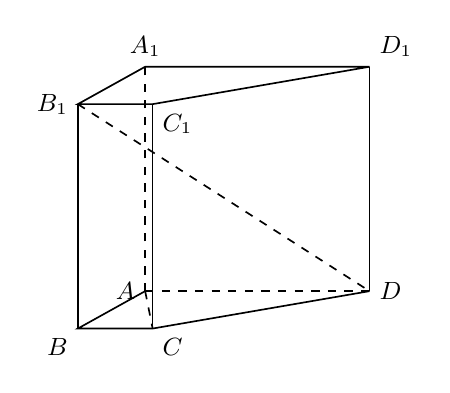
\begin{tikzpicture}[scale=0.95, font=\small, line width=0.6pt]
  \coordinate (A)  at (0,0);
  \coordinate (D)  at (3,0);
  \coordinate (B)  at (-0.9,-0.5);
  \coordinate (C)  at (0.1,-0.5);
  \coordinate (A1) at (0,3);
  \coordinate (D1) at (3,3);
  \coordinate (B1) at (-0.9,2.5);
  \coordinate (C1) at (0.1,2.5);

  % 可见棱
  \draw (A) -- (B) -- (C) -- (D);
  \draw (A1) -- (B1) -- (C1) -- (D1) -- cycle;
  \draw (B) -- (B1);
  \draw (C) -- (C1);
  \draw (D) -- (D1);

  % 不可见棱
  \draw[dashed] (A) -- (A1);
  \draw[dashed] (A) -- (D);
  \draw[dashed] (A) -- (C);
  \draw[dashed] (B1) -- (D);

  \node[left] at (A) {$A$};
  \node[right] at (D) {$D$};
  \node[below left] at (B) {$B$};
  \node[below right] at (C) {$C$};
  \node[above] at (A1) {$A_1$};
  \node[above right] at (D1) {$D_1$};
  \node[left] at (B1) {$B_1$};
  \node[below right] at (C1) {$C_1$};
\end{tikzpicture}
\end{center}
\nopagebreak[4]
\Needspace{4\baselineskip}
\textbf{解析}
\Needspace{5\baselineskip}
\textbf{（1）} 以 $A$ 为原点，$AD$ 为 $x$ 轴，$AB$ 为 $y$ 轴，$AA_1$ 为 $z$ 轴建立空间直角坐标系。设 $AB=t$，则
\nopagebreak[4]
\[A(0,0,0),\quad D(3,0,0),\quad B(0,t,0),\quad C(1,t,0).\]
\Needspace{5\baselineskip}
由 $AC\perp BD$，
\nopagebreak[4]
\[\overrightarrow{AC}\cdot\overrightarrow{BD}=(1,t,0)\cdot(3,-t,0)=3-t^2=0,\]
\Needspace{5\baselineskip}
故 $t=\sqrt3$。于是
\nopagebreak[4]
\[B_1(0,\sqrt3,3),\qquad C_1(1,\sqrt3,3),\qquad D_1(3,0,3).\]
\Needspace{5\baselineskip}
计算
\nopagebreak[4]
\[\overrightarrow{AC}=(1,\sqrt3,0),\qquad
\overrightarrow{B_1D}=(3,-\sqrt3,-3).\]
\Needspace{5\baselineskip}
则
\nopagebreak[4]
\[\overrightarrow{AC}\cdot\overrightarrow{B_1D}
=1\cdot3+\sqrt3\cdot(-\sqrt3)+0\cdot(-3)=3-3=0.\]
所以 $AC\perp B_1D$。

\Needspace{5\baselineskip}
\textbf{（2）} 由（1），
\nopagebreak[4]
\[\overrightarrow{B_1C_1}=(1,0,0),\qquad
\overrightarrow{AC}=(1,\sqrt3,0),\qquad
\overrightarrow{AD_1}=(3,0,3).\]
\Needspace{5\baselineskip}
平面 $ACD_1$ 的一个法向量为
\nopagebreak[4]
\[\boldsymbol n=\overrightarrow{AC}\times\overrightarrow{AD_1}
=(3\sqrt3,-3,-3\sqrt3).\]
\Needspace{5\baselineskip}
设直线 $B_1C_1$ 与平面 $ACD_1$ 所成的角为 $\theta$，则
\nopagebreak[4]
\[\sin\theta=\frac{|\boldsymbol n\cdot\overrightarrow{B_1C_1}|}{|\boldsymbol n|\,|\overrightarrow{B_1C_1}|}
=\frac{3\sqrt3}{3\sqrt7\cdot1}
=\frac{\sqrt3}{\sqrt7}
=\frac{\sqrt{21}}7.\]

\gkanswer{答案（1）：证明见解析。建立空间直角坐标系，由 $\overrightarrow{AC}\cdot\overrightarrow{B_1D}=0$ 得证。}

\gkanswer{答案（2）：$\dfrac{\sqrt{21}}7$。平面 $ACD_1$ 的法向量为 $(3\sqrt3,-3,-3\sqrt3)$，与 $\overrightarrow{B_1C_1}=(1,0,0)$ 夹角的正弦值为 $\dfrac{\sqrt{21}}7$。}

\end{answer}
\begin{answer}
\gksolhead{20}{}

\textbf{题目}：

在平面直角坐标系 $xOy$ 中，将从点 $M$ 出发沿纵、横方向到达点 $N$ 的任一路径称为 $M$ 到 $N$ 的一条“$L$ 路径”。如图所示的路径 $MM_1M_2M_3N$ 与路径 $MN_1N$ 都是 $M$ 到 $N$ 的“$L$ 路径”。某地有三个新建的居民区，分别位于平面 $xOy$ 内三点 $A(3,20)$，$B(-10,0)$，$C(14,0)$ 处。现计划在 $x$ 轴上方区域（包含 $x$ 轴）内的某一点 $P$ 处修建一个文化中心。

（1） 写出点 $P$ 到居民区 $A$ 的“$L$ 路径”长度最小值的表达式（不要求证明）；

（2） 若以原点 $O$ 为圆心，半径为 $1$ 的圆的内部是保护区，“$L$ 路径”不能进入保护区，请确定点 $P$ 的位置，使其到三个居民区的“$L$ 路径”长度之和最小。
\nopagebreak[4]
\begin{center}% 2013 湖南卷理科第 20 题：L 路径示意图（TikZ 矢量重绘）。
% 折线 M-M1-M2-M3-N-N1-M 中，MM1、M2M3、NN1 为横向，M1M2、M3N、N1M 为纵向。
\begin{tikzpicture}[scale=0.85, font=\small, line width=0.6pt]
  \draw[->] (-0.5,0) -- (6.6,0) node[right] {$x$};
  \draw[->] (0,-0.5) -- (0,4.9) node[above] {$y$};
  \node[below left] at (0,0) {$O$};

  \coordinate (M)  at (1.5,4.0);
  \coordinate (M1) at (5.5,4.0);
  \coordinate (M2) at (5.5,2.6);
  \coordinate (M3) at (3.6,2.6);
  \coordinate (N)  at (3.6,1.0);
  \coordinate (N1) at (1.5,1.0);

  \draw (M) -- (M1) -- (M2) -- (M3) -- (N) -- (N1) -- cycle;

  \node[left] at (M) {$M$};
  \node[right] at (M1) {$M_1$};
  \node[right] at (M2) {$M_2$};
  \node[left] at (M3) {$M_3$};
  \node[below] at (N) {$N$};
  \node[left] at (N1) {$N_1$};
\end{tikzpicture}
\end{center}
\nopagebreak[4]
\Needspace{4\baselineskip}
\textbf{解析}
\Needspace{5\baselineskip}
\textbf{（1）} 设 $P(x,y)$，其中 $y\geqslant0$。沿纵、横方向从 $P$ 到 $A(3,20)$ 的任一条“$L$ 路径”的长度都等于横向位移与纵向位移之和，故最小值为
\nopagebreak[4]
\[|x-3|+|y-20|.\]

\Needspace{5\baselineskip}
\textbf{（2）} 对任意 $P(x,y)$，任一条“$L$ 路径”的长度不小于相应的曼哈顿距离，因此
\nopagebreak[4]
\[d(P,A)\geqslant|x-3|+|y-20|,\quad
d(P,B)\geqslant|x+10|+y,\quad
d(P,C)\geqslant|x-14|+y.\]
\Needspace{5\baselineskip}
记
\nopagebreak[4]
\[S(x)=|x-3|+|x+10|+|x-14|.\]
\Needspace{5\baselineskip}
数轴上的绝对值距离和在三数中位数处取得最小值，故
\nopagebreak[4]
\[S(x)\geqslant S(3)=0+13+11=24,\]
且等号仅在 $x=3$ 时成立；进一步有 $S(x)\geqslant24+|x-3|$。

\Needspace{5\baselineskip}
先设 $0\leqslant y\leqslant20$。三条路径长度之和 $F$ 满足
\nopagebreak[4]
\[F\geqslant S(x)+20+y\geqslant44+y+|x-3|.\]

\Needspace{5\baselineskip}
若 $y\geqslant1$，则
\nopagebreak[4]
\[F\geqslant45+|x-3|\geqslant45,\]
\Needspace{5\baselineskip}
当 $x=3$ 且 $y=1$ 时取到 $45$：此时到 $A$ 的路径长 $19$，到 $B$ 的路径长 $13+1=14$，到 $C$ 的路径长 $11+1=12$，总和为
\nopagebreak[4]
\[19+14+12=45.\]
这些路径可沿直线 $y=1$ 横向行进，而直线 $y=1$ 与保护圆相切，不进入圆的内部。

\Needspace{5\baselineskip}
若 $0\leqslant y<1$，则 $P$ 到 $B$，$C$ 中至少一个的路径必须从 $y$ 轴一侧穿到另一侧。由于不能进入单位圆的内部，穿越 $y$ 轴时的纵坐标绝对值至少为 $1$；路径从高度 $y<1$ 出发、最后回到高度 $0$，至少要先上升到高度 $1$ 再下降，故比曼哈顿下界至少多出
\nopagebreak[4]
\[2(1-y).\]
\Needspace{5\baselineskip}
于是
\nopagebreak[4]
\[F\geqslant44+y+|x-3|+2(1-y)
=46-y+|x-3|>45.\]
\Needspace{5\baselineskip}
若 $y>20$，则 $d(P,A)\geqslant y-20$，而 $d(P,B)$，$d(P,C)$ 均不小于 $y$，从而
\nopagebreak[4]
\[F\geqslant S(x)+3y-20\geqslant24+3y-20>64>45.\]

综上，当且仅当 $P(3,1)$ 时，到三个居民区的“$L$ 路径”长度之和最小，最小值为 $45$。

\gkanswer{答案（1）：$|x-3|+|y-20|$。}

\gkanswer{答案（2）：$P(3,1)$。此时三条“$L$ 路径”长度之和为 $45$，且为最小值。}

\end{answer}
\begin{answer}
\gksolhead{21}{}

\textbf{题目}：

过抛物线 $E:x^2=2py$（$p>0$）的焦点 $F$ 作斜率分别为 $k_1$，$k_2$ 的两条不同的直线 $l_1$，$l_2$，且 $k_1+k_2=2$，$l_1$ 与 $E$ 相交于点 $A$，$B$，$l_2$ 与 $E$ 相交于点 $C$，$D$。以 $AB$，$CD$ 为直径的圆 $M$，圆 $N$（$M$，$N$ 为圆心）的公共弦所在的直线记为 $l$。

（1） 若 $k_1>0$，$k_2>0$，证明：$\overrightarrow{FM}\cdot\overrightarrow{FN}<2p^2$；

（2） 若点 $M$ 到直线 $l$ 的距离的最小值为 $\dfrac{7\sqrt5}{5}$，求抛物线 $E$ 的方程。

\Needspace{4\baselineskip}
\textbf{解析}
\Needspace{5\baselineskip}
抛物线 $E:x^2=2py$ 的焦点为 $F\left(0,\dfrac p2\right)$。过 $F$ 且斜率为 $k$ 的直线为
\nopagebreak[4]
\[y=kx+\frac p2.\]
\Needspace{5\baselineskip}
与 $x^2=2py$ 联立：
\nopagebreak[4]
\[x^2=2p\left(kx+\frac p2\right)=2pkx+p^2,\]
\Needspace{5\baselineskip}
即
\nopagebreak[4]
\[x^2-2pkx-p^2=0.\]
\Needspace{5\baselineskip}
设两个交点的横坐标为 $x_1$，$x_2$，则
\nopagebreak[4]
\[x_1+x_2=2pk,\qquad x_1x_2=-p^2.\]
\Needspace{5\baselineskip}
弦的中点（圆心）为
\nopagebreak[4]
\[\left(pk,\;p\left(k^2+\frac12\right)\right).\]
\Needspace{5\baselineskip}
以该弦为直径的圆的方程为
\nopagebreak[4]
\[(x-x_1)(x-x_2)+(y-y_1)(y-y_2)=0,\]
\Needspace{5\baselineskip}
即
\nopagebreak[4]
\[x^2+y^2-(x_1+x_2)x-(y_1+y_2)y+x_1x_2+y_1y_2=0.\]
\Needspace{5\baselineskip}
由 $y_i=kx_i+\dfrac p2$ 得
\nopagebreak[4]
\[y_1+y_2=k(x_1+x_2)+p=2pk^2+p,\]
\nopagebreak[4]
\[y_1y_2=k^2x_1x_2+\frac{kp}{2}(x_1+x_2)+\frac{p^2}{4}
=-k^2p^2+k^2p^2+\frac{p^2}{4}=\frac{p^2}{4}.\]
\Needspace{5\baselineskip}
故圆的方程可写成
\nopagebreak[4]
\[x^2+y^2-2pk\,x-(2pk^2+p)y-\frac{3p^2}{4}=0.\]
\Needspace{5\baselineskip}
对 $k=k_1$ 与 $k=k_2$ 的两圆相减，常数项相同，得公共弦所在直线
\nopagebreak[4]
\[-2p(k_1-k_2)x-2p(k_1^2-k_2^2)y=0,\]
\Needspace{5\baselineskip}
即
\nopagebreak[4]
\[x+(k_1+k_2)y=0.\]
\Needspace{5\baselineskip}
由 $k_1+k_2=2$，直线 $l$ 的方程为
\nopagebreak[4]
\[x+2y=0.\]

\Needspace{5\baselineskip}
\textbf{（1）} 两圆圆心分别为
\nopagebreak[4]
\[M\left(pk_1,p\left(k_1^2+\frac12\right)\right),\qquad
N\left(pk_2,p\left(k_2^2+\frac12\right)\right).\]
\Needspace{5\baselineskip}
于是
\nopagebreak[4]
\[\overrightarrow{FM}=\left(pk_1,pk_1^2\right),\qquad
\overrightarrow{FN}=\left(pk_2,pk_2^2\right),\]
\nopagebreak[4]
\[\overrightarrow{FM}\cdot\overrightarrow{FN}
=p^2\left(k_1k_2+k_1^2k_2^2\right)
=p^2t(1+t),\]
\Needspace{5\baselineskip}
其中 $t=k_1k_2$。由 $k_1>0$，$k_2>0$ 及 $k_1+k_2=2$，得
\nopagebreak[4]
\[0<t\leqslant\left(\frac{k_1+k_2}{2}\right)^2=1.\]
\Needspace{5\baselineskip}
又 $l_1$，$l_2$ 不同，故 $k_1\neq k_2$，从而 $t<1$。于是
\nopagebreak[4]
\[t(1+t)<1\cdot(1+1)=2,\]
\Needspace{5\baselineskip}
所以
\nopagebreak[4]
\[\overrightarrow{FM}\cdot\overrightarrow{FN}<2p^2.\]

\Needspace{5\baselineskip}
\textbf{（2）} 点 $M$ 到直线 $l:x+2y=0$ 的距离为
\nopagebreak[4]
\[d=\frac{\left|pk_1+2p\left(k_1^2+\frac12\right)\right|}{\sqrt5}
=\frac{p\left|2k_1^2+k_1+1\right|}{\sqrt5}.\]
\Needspace{5\baselineskip}
二次函数
\nopagebreak[4]
\[2k_1^2+k_1+1=2\left(k_1+\frac14\right)^2+\frac78\]
\Needspace{5\baselineskip}
恒正，且最小值为 $\dfrac78$（此时 $k_1=-\dfrac14$，$k_2=\dfrac94$，两直线不同）。故
\nopagebreak[4]
\[d_{\min}=\frac{p}{\sqrt5}\cdot\frac78=\frac{7p}{8\sqrt5}.\]
\Needspace{5\baselineskip}
由题设 $d_{\min}=\dfrac{7\sqrt5}{5}$：
\nopagebreak[4]
\[\frac{7p}{8\sqrt5}=\frac{7\sqrt5}{5}
\Longrightarrow p=\frac{8\sqrt5\cdot\sqrt5}{5}=8.\]
\Needspace{5\baselineskip}
所以抛物线 $E$ 的方程为
\nopagebreak[4]
\[x^2=16y.\]

\gkanswer{答案（1）：证明见解析。$\overrightarrow{FM}\cdot\overrightarrow{FN}=p^2k_1k_2(1+k_1k_2)$，由 $0<k_1k_2<1$ 得证。}

\gkanswer{答案（2）：$x^2=16y$。公共弦所在直线为 $x+2y=0$，点 $M$ 到它的距离最小值为 $\dfrac{7p}{8\sqrt5}$，令其等于 $\dfrac{7\sqrt5}{5}$ 得 $p=8$。}

\end{answer}
\begin{answer}
\gksolhead{22}{}

\textbf{题目}：

已知 $a>0$，函数 $f(x)=\dfrac{|x-a|}{x+2a}$。

（1） 记 $f(x)$ 在区间 $[0,4]$ 上的最大值为 $g(a)$，求 $g(a)$ 的表达式；

（2） 是否存在 $a$，使函数 $y=f(x)$ 在区间 $(0,4)$ 内的图象上存在两点，在该两点处的切线相互垂直？若存在，求 $a$ 的取值范围；若不存在，请说明理由。

\Needspace{4\baselineskip}
\textbf{解析}
\textbf{（1）} 当 $x\in[0,4]$ 时，$x+2a>0$。

\Needspace{5\baselineskip}
若 $0\leqslant x\leqslant a$，则
\nopagebreak[4]
\[f(x)=\frac{a-x}{x+2a}=-1+\frac{3a}{x+2a},\]
\Needspace{5\baselineskip}
随 $x$ 增大而减小；若 $x\geqslant a$，则
\nopagebreak[4]
\[f(x)=\frac{x-a}{x+2a}=1-\frac{3a}{x+2a},\]
\Needspace{5\baselineskip}
随 $x$ 增大而增大。因此 $f$ 在 $[0,4]$ 上的最大值只能在端点 $x=0$ 或 $x=4$ 处取得：
\nopagebreak[4]
\[f(0)=\frac12,\qquad
f(4)=\frac{|4-a|}{4+2a}.\]
\Needspace{5\baselineskip}
所以
\nopagebreak[4]
\[g(a)=\max\left\{\frac12,\frac{|4-a|}{4+2a}\right\}.\]
\Needspace{5\baselineskip}
当 $0<a\leqslant4$ 时，
\nopagebreak[4]
\[\frac{4-a}{4+2a}\geqslant\frac12
\Longleftrightarrow 8-2a\geqslant4+2a
\Longleftrightarrow a\leqslant1.\]
\Needspace{5\baselineskip}
当 $a>4$ 时，
\nopagebreak[4]
\[\frac{a-4}{4+2a}<\frac12\]
\Needspace{5\baselineskip}
恒成立。故
\nopagebreak[4]
\[g(a)=\begin{cases}
\dfrac{4-a}{4+2a},&0<a\leqslant1,\\[2mm]
\dfrac12,&a>1.
\end{cases}\]

\Needspace{5\baselineskip}
\textbf{（2）} 当 $x>a$ 时，
\nopagebreak[4]
\[f'(x)=\frac{3a}{(x+2a)^2}>0;\]
\Needspace{5\baselineskip}
当 $0<x<a$ 时，
\nopagebreak[4]
\[f'(x)=-\frac{3a}{(x+2a)^2}<0.\]
\Needspace{5\baselineskip}
同支上两切线斜率同号，不可能垂直。若存在两点处切线互相垂直，必须一点在 $x>a$ 的支上，另一点在 $0<x<a$ 的支上。设其横坐标分别为 $x_1$，$x_2$，其中
\nopagebreak[4]
\[a<x_1<4,\qquad 0<x_2<a.\]
\Needspace{5\baselineskip}
垂直条件为
\nopagebreak[4]
\[\frac{3a}{(x_1+2a)^2}\cdot\left(-\frac{3a}{(x_2+2a)^2}\right)=-1,\]
\Needspace{5\baselineskip}
即
\nopagebreak[4]
\[(x_1+2a)(x_2+2a)=3a.\]
\Needspace{5\baselineskip}
令
\nopagebreak[4]
\[u=x_1+2a,\qquad v=x_2+2a.\]
\Needspace{5\baselineskip}
则
\nopagebreak[4]
\[u\in(3a,4+2a),\qquad v\in(2a,3a),\qquad uv=3a.\]
\Needspace{5\baselineskip}
必要性：由 $u>3a$，$v>2a$ 得
\nopagebreak[4]
\[3a=uv>6a^2\Longrightarrow a<\frac12.\]
\Needspace{5\baselineskip}
充分性：当 $0<a<\dfrac12$ 时，区间 $\left(2a,1\right)$ 非空（因 $2a<1$）。取 $v\in(2a,1)$，令 $u=\dfrac{3a}{v}$。则
\nopagebreak[4]
\[v<1\Longrightarrow u>3a,\qquad
v>2a\Longrightarrow u<\frac{3a}{2a}=\frac32<4+2a,\]
\Needspace{5\baselineskip}
从而
\nopagebreak[4]
\[x_1=u-2a\in(a,4),\qquad x_2=v-2a\in(0,a),\]
且 $uv=3a$，对应的两切线互相垂直。

\Needspace{5\baselineskip}
因此存在这样的 $a$，其取值范围为
\nopagebreak[4]
\[0<a<\frac12.\]

\gkanswer{答案（1）：$g(a)=\begin{cases}\dfrac{4-a}{4+2a},&0<a\leqslant1,\\[2mm]\dfrac12,&a>1.\end{cases}$}

\gkanswer{答案（2）：存在，$0<a<\dfrac12$。两支上切点横坐标记为 $x_1$，$x_2$，垂直条件等价于 $(x_1+2a)(x_2+2a)=3a$。}

\end{answer}